\documentclass{standalone}
\usepackage{tikz}
\usepackage{xcolor}

\usetikzlibrary{decorations.pathmorphing}
\usetikzlibrary{shapes}
\usetikzlibrary{shapes.geometric}


\begin{document}
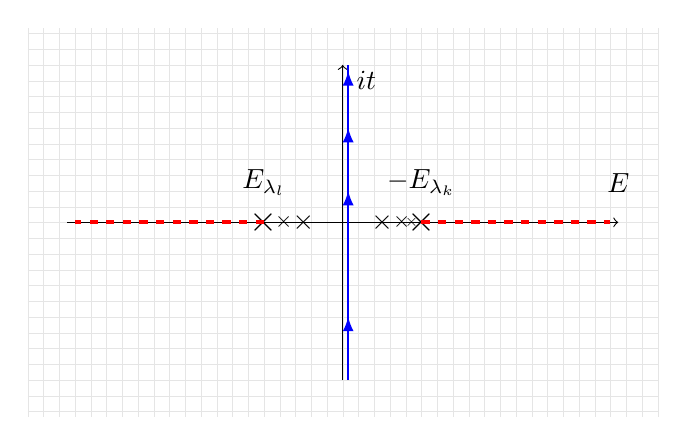
\begin{tikzpicture}
\usetikzlibrary{decorations.markings}
	\draw[gray!20,line width=0.01mm,step=0.2] (-4,-2.472) grid (4, 2.472);

	\draw[->] (0,-2) -- (0,2);  % Axis
	\draw[->] (-3.5,0) -- (3.5,0);   

	\draw node[scale=1.3] at (-1,0) {$\times$}; % Pole
	\draw node[scale=1.3] at (1,0) {$\times$}; % Pole
	\draw node[scale=1] at (-0.5,0) {$\times$}; % Pole
	\draw node[scale=1] at (0.5,0) {$\times$}; % Pole
	\draw node[scale=0.8] at (-0.75,0) {$\times$}; % Pole
	\draw node[scale=0.8] at (0.75,0) {$\times$}; % Pole
	\draw node[scale=0.6] at (0.875,0) {$\times$}; % Pole
	
	\draw[dashed, red, line width=0.5 mm] (1,0) -- (3.4,0);
	\draw[dashed, red, line width=0.5 mm] (-1,0) -- (-3.4,0);
	
	\node at (3.5,0.5) {\textcolor{black}{ $E$}};
	\node at (1,0.5) {\textcolor{black}{ $-E_{\lambda_k}$}};
	\node at (-1,0.5) {\textcolor{black}{ $E_{\lambda_l}$}};
\node at (0.3,1.8) {\textcolor{black}{ $i t$}};
	
	% Contour line
	\draw[thick,blue,xshift=2pt,
	decoration={ markings,  % This schema allows for fine-tuning the positions of arrows
		mark=at position 0.2 with {\arrow{latex}}, 
		mark=at position 0.6 with {\arrow{latex}},
		mark=at position 0.8 with {\arrow{latex}}, 
		mark=at position 0.98 with {\arrow{latex}}}, 
	postaction={decorate}]
	(0,-2) -- (0,2);
\end{tikzpicture}
\end{document}